\chapter{Polyhedra}\label{polyhedra}

\iffalse
\setcounter{section}{-1}
% New Section %%%%%%%%%%%%%%%%%%%%%%%%%%%%%%%%%%%%%%%%%%%%%%%%
\section{Mathematical Outcome}\label{sec:PolyhedraOutcome}
%%%%%%%%%%%%%%%%%%%%%%%%%%%%%%%%%%%%%%%%%%%%%%%%%%%%%%%%%%%%%%
\fi

% New Section %%%%%%%%%%%%%%%%%%%%%%%%%%%%%%%%%%%%%%%%%%%%%%%%
\section{Funny Dice}\label{sec:FunnyDice}
%%%%%%%%%%%%%%%%%%%%%%%%%%%%%%%%%%%%%%%%%%%%%%%%%%%%%%%%%%%%%%

%%%%%%%%%%%%%%%%%%%%%%%%%%%%%%%%%%%%%%%%%%%%%%%%%%%%%%%%%%%%%%
\subsection{Entrance Activity: Dice}

\Instr{  Make sure to bring sufficient copies of the handout ``D4.pdf'' and enough scissors to go around for this activity.}

Dice are certainly familiar items from the world around us.  There are games that can be played with dice alone, and there are many games that use dice to add an element of randomness -- for instance in Monopoly, each player rolls the dice when it's their turn and that determines how many positions their token moves.  A single die is a random number generator with possible values from 1 to 6.

\centerline{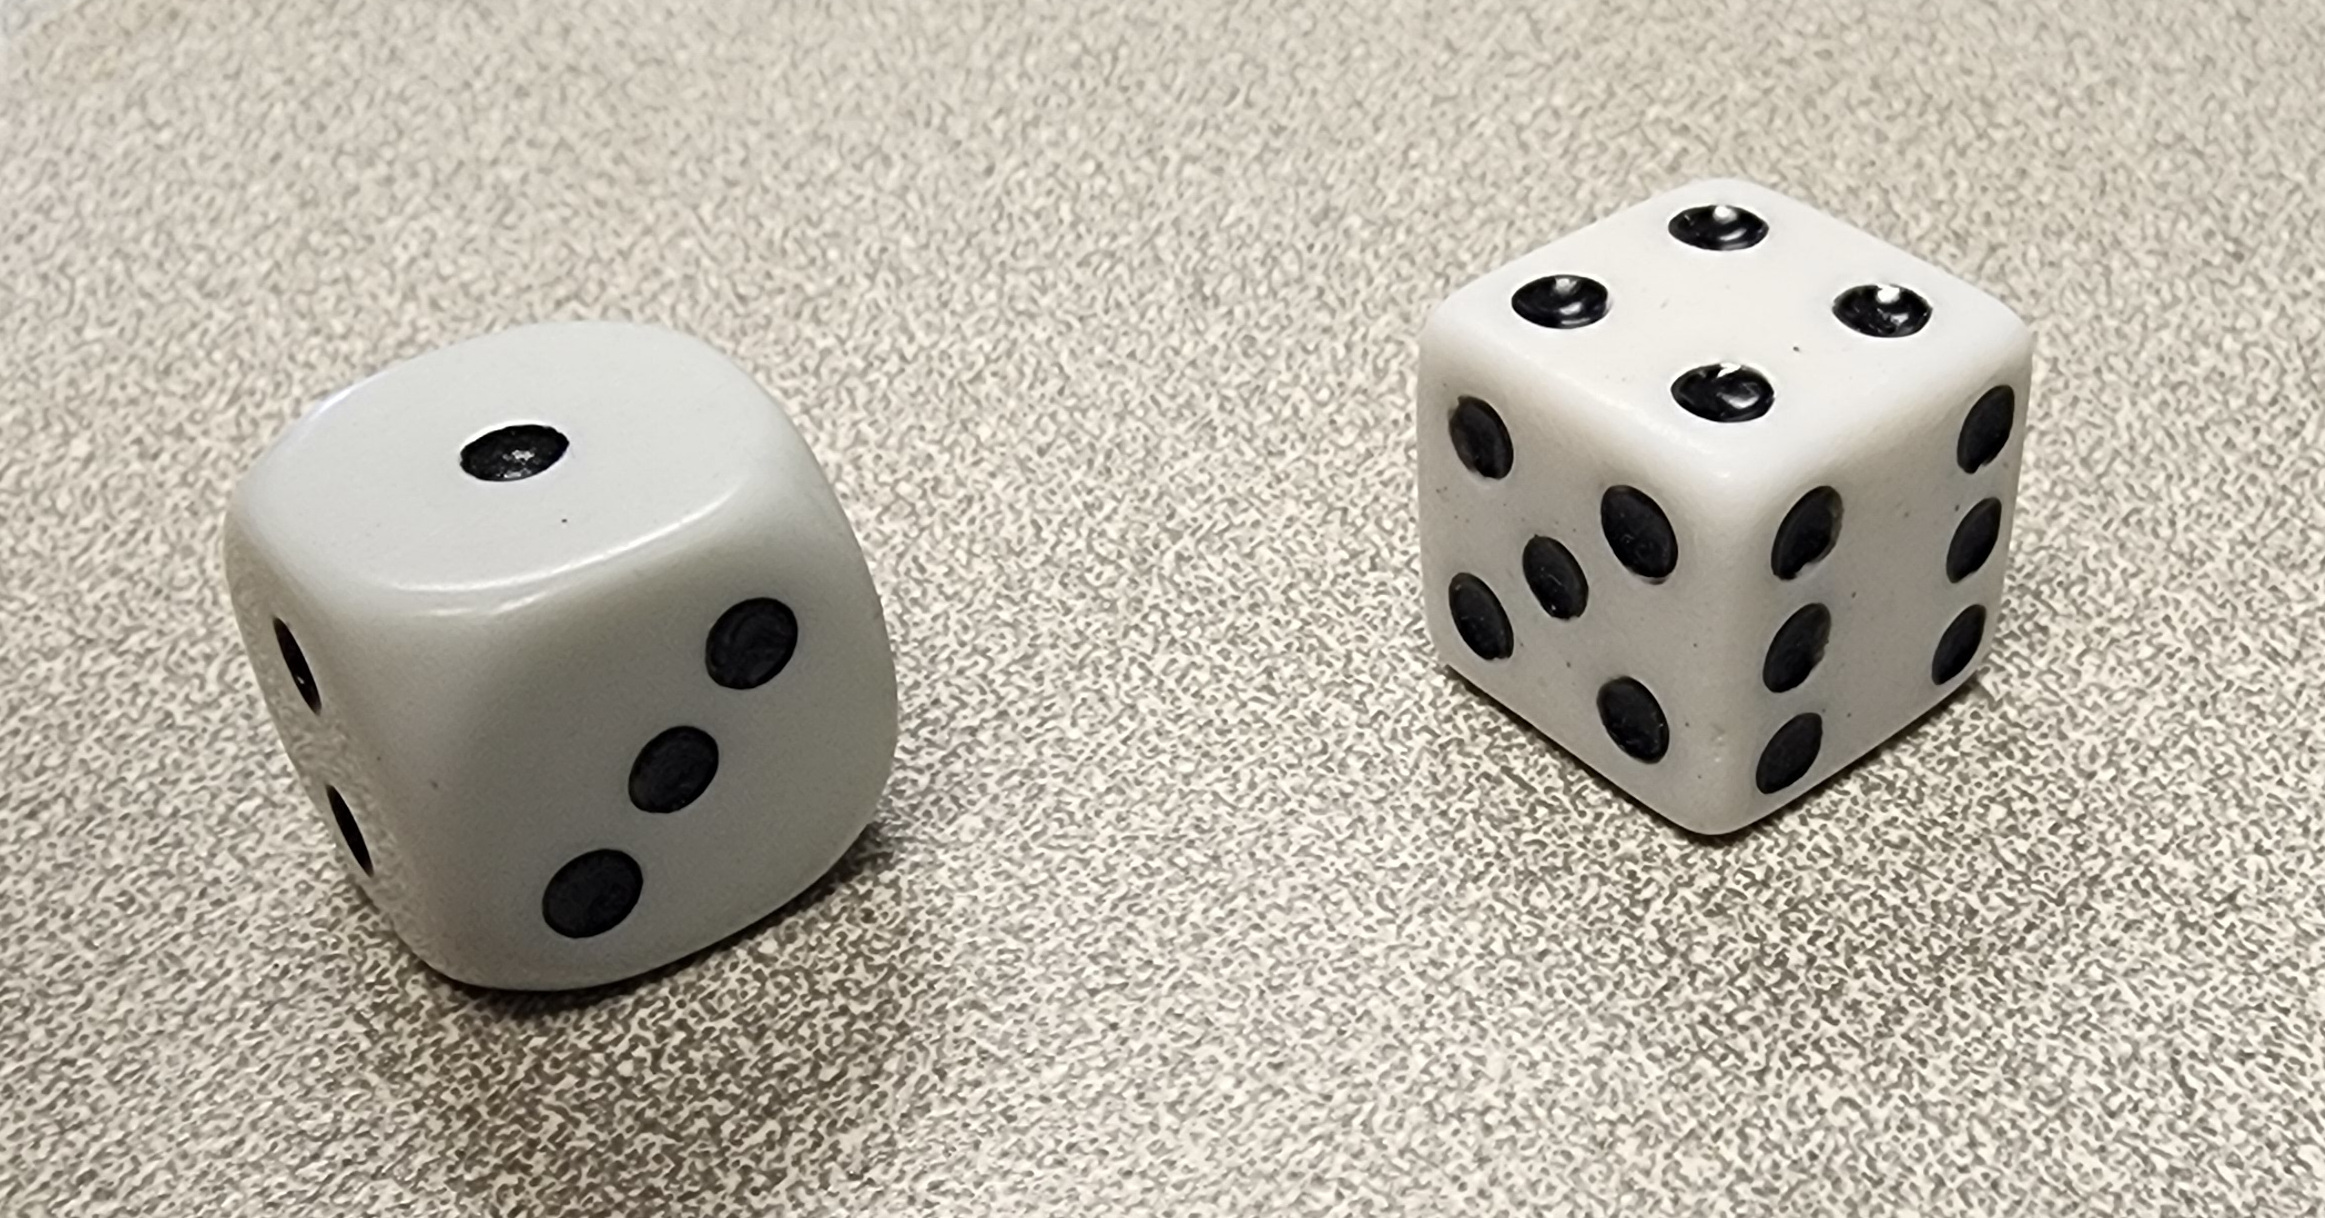
\includegraphics[scale=.1]{images/dice.jpg}}

Often (when numbers larger than 6 are required), we use two die.  That gets us numbers from 2 to 12, but there's a funny consequence -- some numbers are more likely to come up than others.

There are 6 different ways that you can roll a 7 with two die.  Can you list them?
\bigskip

\centerline{ \begin{tabular}{c|c} 
\bigstrut die 1 & die 2 \\ \hline
\bigstrut & \\ \hline
\bigstrut & \\ \hline
\bigstrut & \\ \hline
\bigstrut & \\ \hline
\bigstrut & \\ \hline
\bigstrut & \\ 
\end{tabular}
}
\bigskip

How many ways can you roll an 11?

\vspace{.5in}

So, on average, how many 7's would you see for each 11 if you were rolling the dice a bunch of times?

\vspace{.5in}

If we want ``dice-like things'' (random number generators that give equal weight to the options) we'll need solid geometric objects that are nice and regular, but that have different numbers of sides.  Here are a few examples:

\centerline{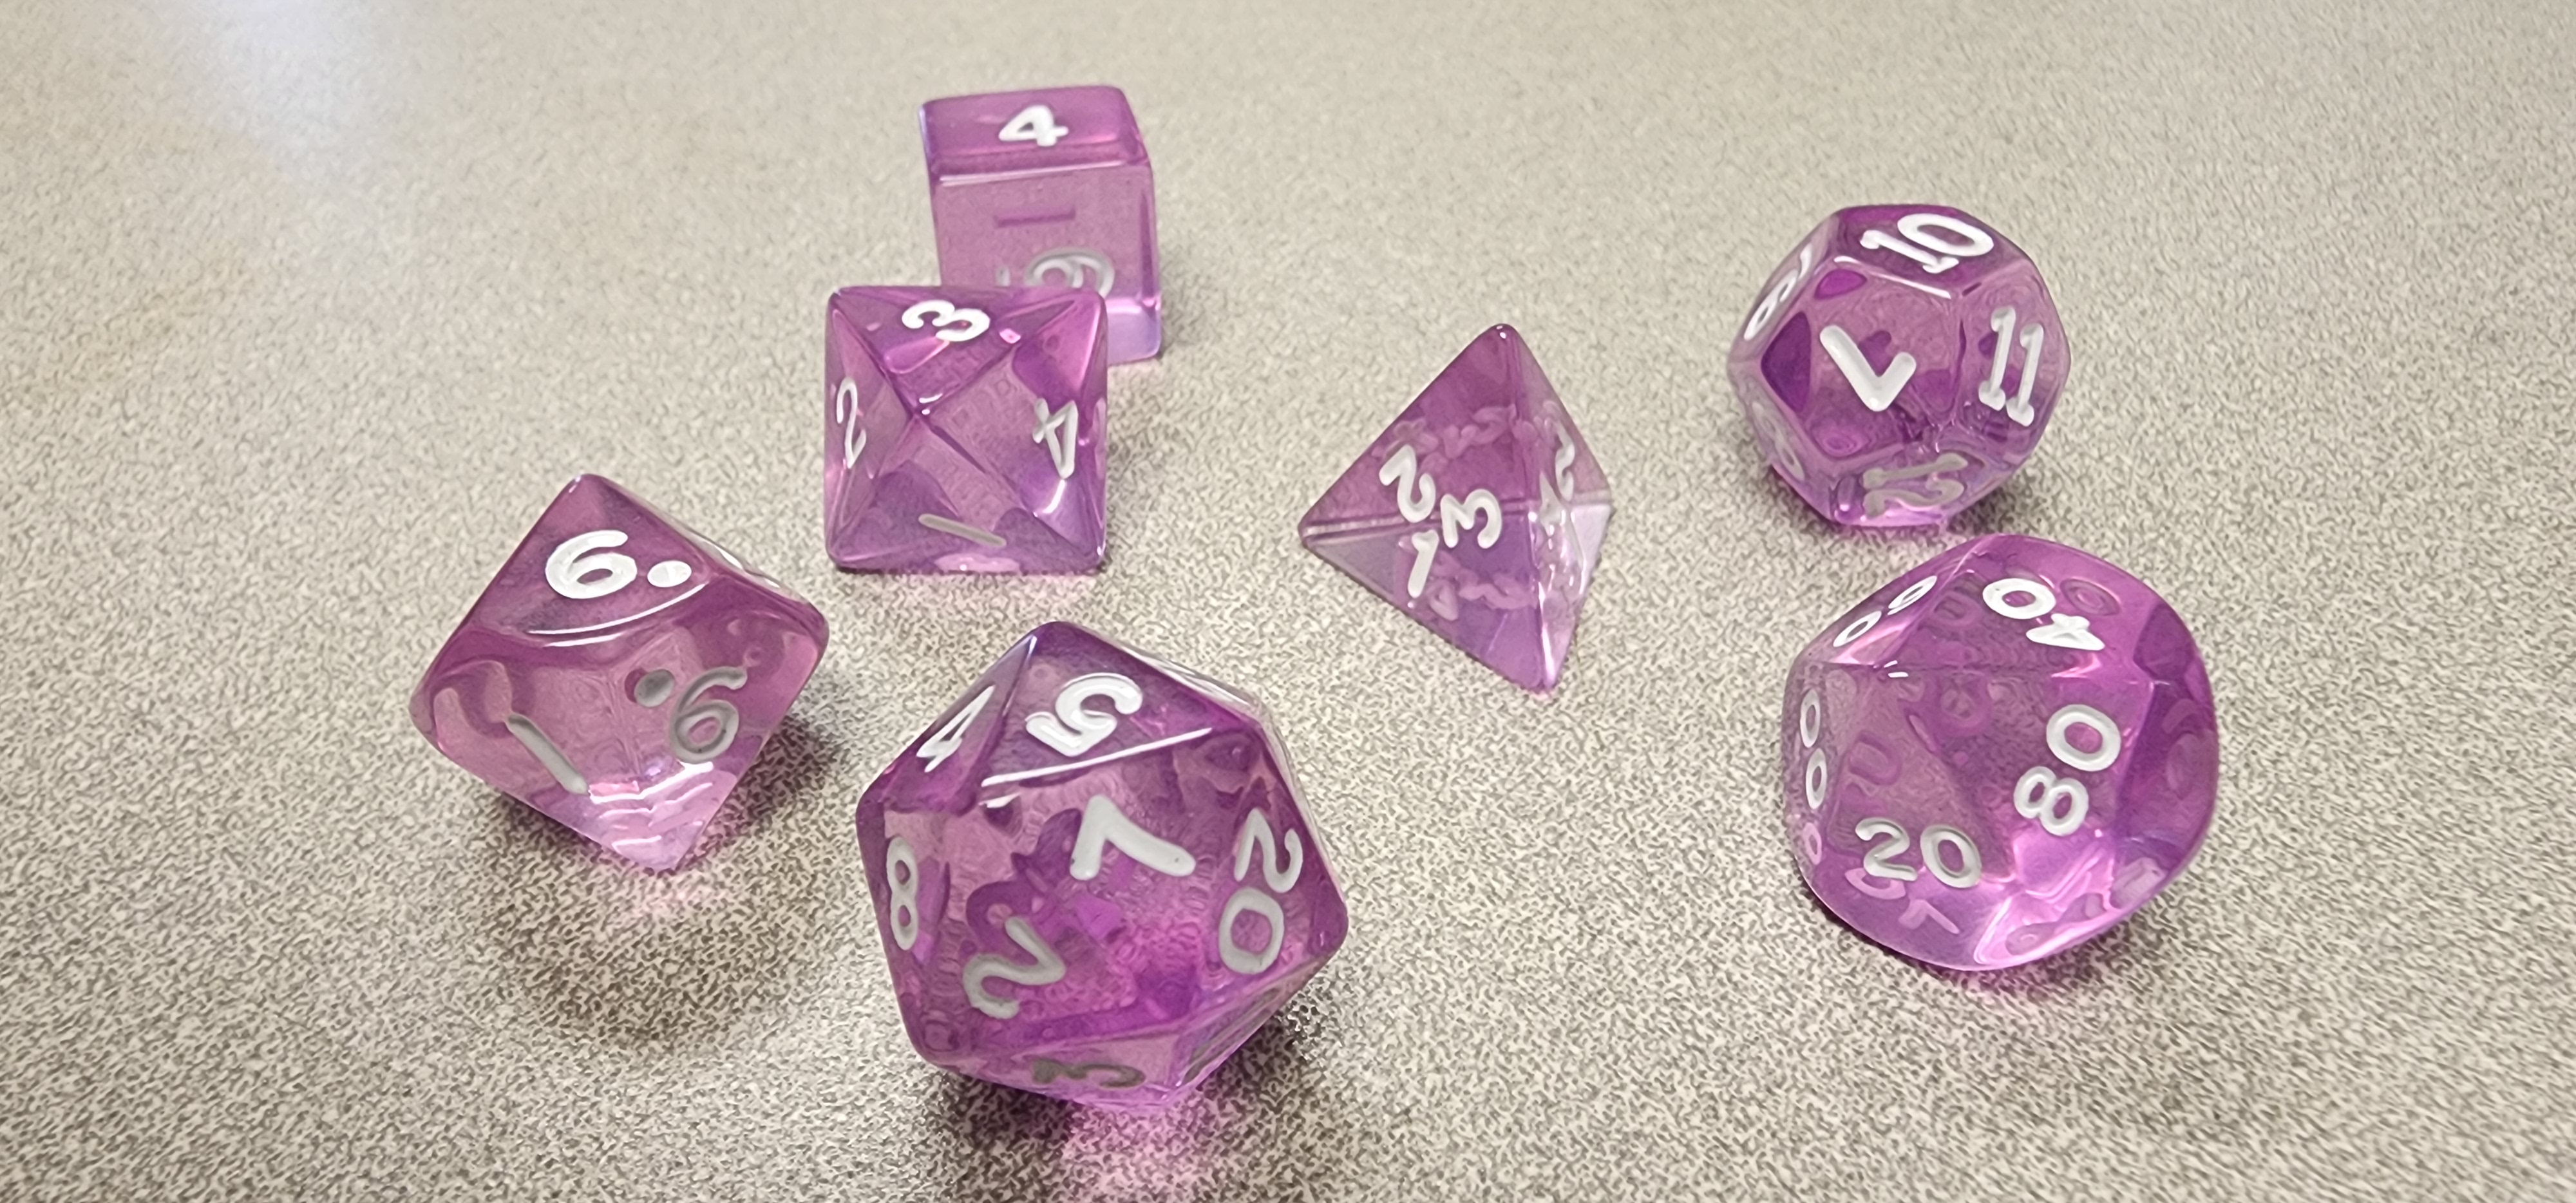
\includegraphics[scale=.1]{images/fancy_dice.jpg}}
\bigskip

There are other options, but a good place to start is with the five Platonic solids.  Apparently, Plato (an ancient Greek philosopher) knew about these five, extremely regular, solid objects.  The smallest platonic solid is known as a tetrahedron -- gamers call it D4.  

The pyramids that can be found in Egypt and a few other places around the world have triangular sides, but square bases.  Can you imagine what it would look like if a pyramid's base was also a triangle?  

You're going to make your own D4 today. The style of construction method we'll use is called {\em plaiting}.  Carefully cut out the two strips from the handout.  Pre-crease the edges between triangles, then weave the two strips together.  It may seem hard at first, but the pattern is just over-under-over-under.  Be sure that the markings are on the outside when you are finished!

\vspace{.5in}

Notice that there are 3 edges on each triangle (duh!) and since there are 4 triangles that makes a total of $3 \cdot 4 \; = \; 12$ edges.  But there are only 6 edges on the D4 we just made.  Can you explain why?

\wbvfill

\newpage

\subsection{Activity: Why Only Five?}

\Instr{  In the ``images'' directory are pdfs of templates for constructing an icosahedron and a dodecahedron.  If this activity stretches over two class periods there may be time for students to actually construct them, and hence it might be nice to bring a supply of copies of the templates (ideally on heavier paper) and scissors and glue. }

Let's start by thinking a bit about why cubes are the perfect 3-d shape to use for dice.  Cubes are made up of squares, but you could make an imperfect cube out of rectangles -- think of a brick.  Explain why tossing a brick would be a poor choice for generating random numbers.

\vspace{1in}

It seems we should build our ``fancy'' dice using faces that are {\bf regular} like a square.  The regular polygons that can be used are:

\begin{enumerate}
    \item equilateral triangles
    \item squares
    \item regular pentagons
\end{enumerate}

Of course, triangles are the smallest possible polygons, but what about on the big side?  Can anyone come up with a reason why we couldn't make a 3-d object with hexagons, heptagons, octagons, etc. as the sides?

\vspace{1in}

A tool we can use to think carefully about polyhedra (that's the generic term for a solid with many sides) is the so-called {\em net} of the polyhedron.  There are generally many different nets for a given polyhedron.  Here's one for a cube:
\bigskip

\centerline{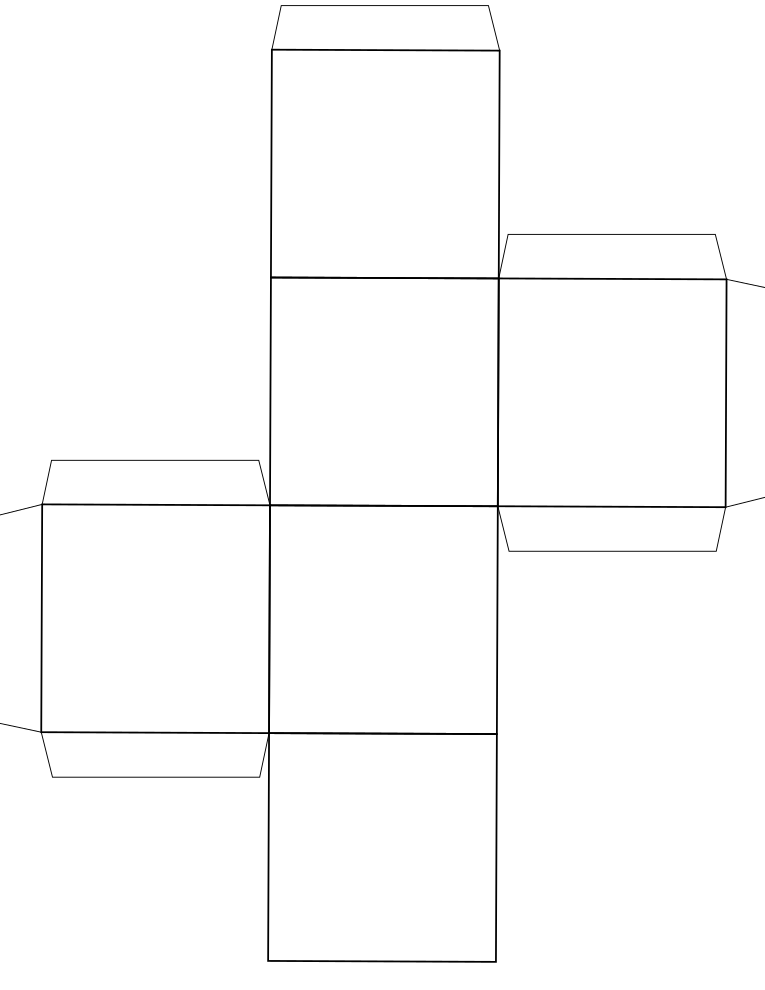
\includegraphics[scale=.25]{images/cube-net.png}}

Officially, a net wouldn't include the little tabs that are meant for gluing the model together. But, as you can probably tell from the example, the net of a solid is a flat template that can be folded up to cover the exterior of the solid.

Which of the following is a net for the tetrahedron?
\bigskip

\centerline{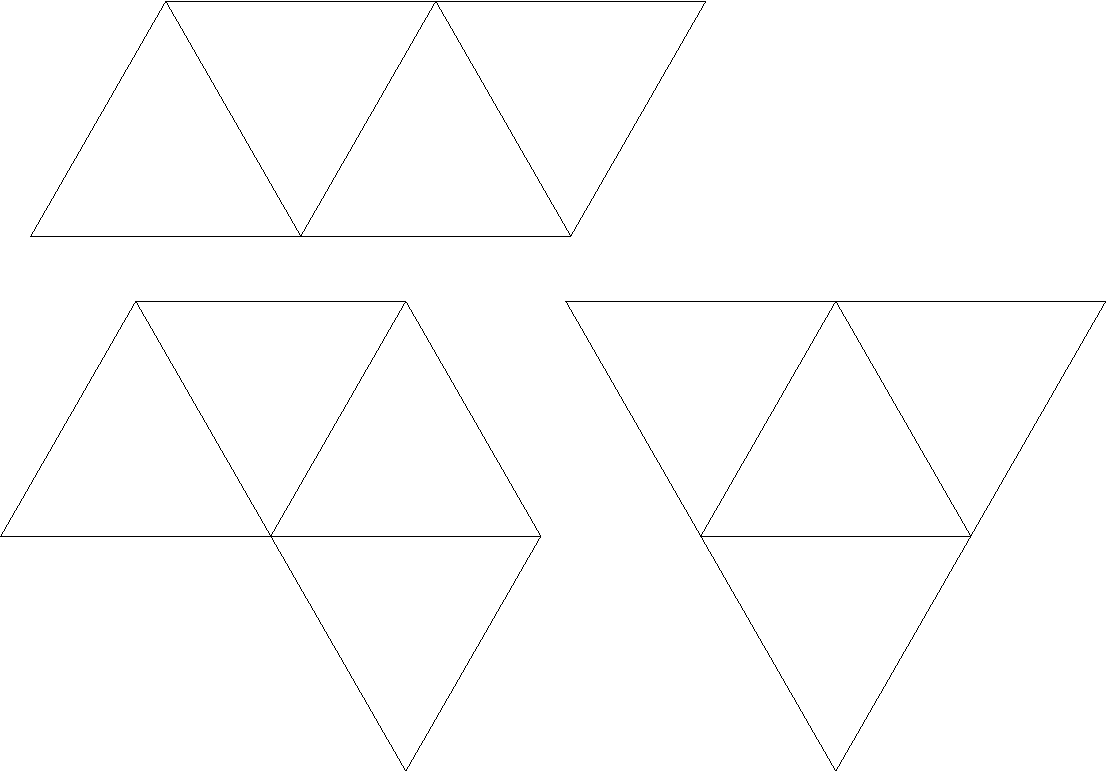
\includegraphics[scale=.25]{images/tetrahedron_nets.png}}
\bigskip

A quick way to rule out a potential net is to count how many polygons will meet at each corner.  In a tetrahedron, exactly $3$ triangles meet at each corner. Now do you see which one of the above is impossible?

\wbvfill

Let's recap for a minute.  We're trying to figure out how to make ``fancy'' dice that will have a different number of sides than a cube does.  We know that the faces of our dice will have 3, 4, or 5 sides.  Finally, it seems that the number of faces that meet at a corner is important.  Some of you may know about D8, D12 and D20, but the only solids we've discovered together so far are D4 and D6 -- the tetrahedron and the cube.

Let's collect what we've found so far in a table.

Also, let's (please!) agree to use the following abbreviations:

$F =$ the number of faces on the object.

$C =$ the number of corners on the object.

$F/C =$ the number of faces that meet at a corner.

$C/F =$ the number of corners on each face.

$E =$ the number of edges.
\bigskip

\begin{tabular}{r|c|c|c|c|c} 
\bigstrut name & $F$ & $C$ & $F/C$ & $C/F$ & $E$ \\ \hline
\bigstrut tetrahedron & \hstrut & \hstrut & \hstrut & \hstrut & \hstrut \\ \hline
\bigstrut cube & & & & & 
\end{tabular}

\wbnewpage

Near the beginning of this activity we asked, ``Can anyone come up with a reason why we couldn't make a 3-d object with hexagons, heptagons, octagons, etc. as the sides?''  There are two facts that explain the situation.

\begin{itemize}
    \item[{\bf Fact 1:}] You have to have 3 or more faces meeting at a corner. \newline
    (What would it look like if only two faces (of whatever type (sorry about the nested parentheses)) met at a corner?)
    \item[{\bf Fact 2:}] The sum of the angles on the faces that meet at a corner must be less than $360^\circ$ \newline
\end{itemize}

Fact 2 might best be illustrated by an example.  What would it look like, if instead of having 3 squares meet at a corner, we tried to get 4 squares to meet at a corner. (Hint: look down.)

The angle on the corner of a hexagon is $120^\circ$ and if $3$ of them met at a corner, we'd get a tiling of the plane -- not a polyhedron of any sort.  Here's a hard question: what is the angle found on the corner of a regular pentagon, and how many regular pentagons could meet at the corners of a polyhedron?

\vspace{1in}

Alright then! If a polyhedron has squares as its faces there must be \underline{\hstrut} of them meeting at a corner, and that gets us a cube!  If a polyhedron has regular pentagons as its faces there must also be \underline{\hstrut} of them meeting at a corner, and that beast is called the dodecahedron.  We'll come back to that!

What are the possible values of $F/C$ if the faces are triangles?

\vspace{.5in} 

Here's a bit more of the table we started previously.

\bigskip
\setlength{\tabcolsep}{18pt}
\begin{tabular}{r|c|c|c|c|c} 
\bigstrut name        & $F$ & $C$ & $F/C$ & $C/F$ & $E$ \\ \hline
\bigstrut tetrahedron & 4   & 4   & 3     & 3     & 6 \\ \hline
\bigstrut cube        & 6   & 8   & 3     & 4     & 12 \\ \hline
\bigstrut octahedron  &     &     & 4     & 3     &   \\
\end{tabular}
\bigskip

The new object in the row that's been added is called the {\em octahedron} and the entries that are pre-filled tell us that it's made of triangles with 4 of them meeting at a corner. A little thinking about etymology will probably let you guess how many faces it has.  Rather than building a model, we'll just try to get you to visualize this solid in your mind's eye.  Imagine taking two (Egyptian-style, square based) pyramids and gluing them together along their square bases -- the resulting thing would only have triangles (8 of them!) visible on the outside and there would be $4$ meeting at each corner.

\Instr{  It's possible that students might ask about gluing tetrahedra together in a similar fashion.  Of course that gets us 6 faces, and we've already got cubes\textellipsis Ask them about regularity - does the solid formed out of two triangular pyramids glued together at their bases have the same number of faces meeting at each corner?  This inquiry also leads to the interesting family of bi-pyramidal dice.}

With that visualization you should now be able to fill out the remaining entries in the octahedron row.

There are two remaining objects in this list of the $5$ Platonic solids we're trying to build.
The {\em dodecahedron} (aka D12) and the {\em icosahedron} (aka D20).  One of them is built of 5-sided polygons meeting 3 at a corner.  The other is made of 3-sided polygons meeting 5 at a corner.  Isn't that weird switching-around of 3's and 5's interesting?

Here's a net for the dodecahedron:
\bigskip

\centerline{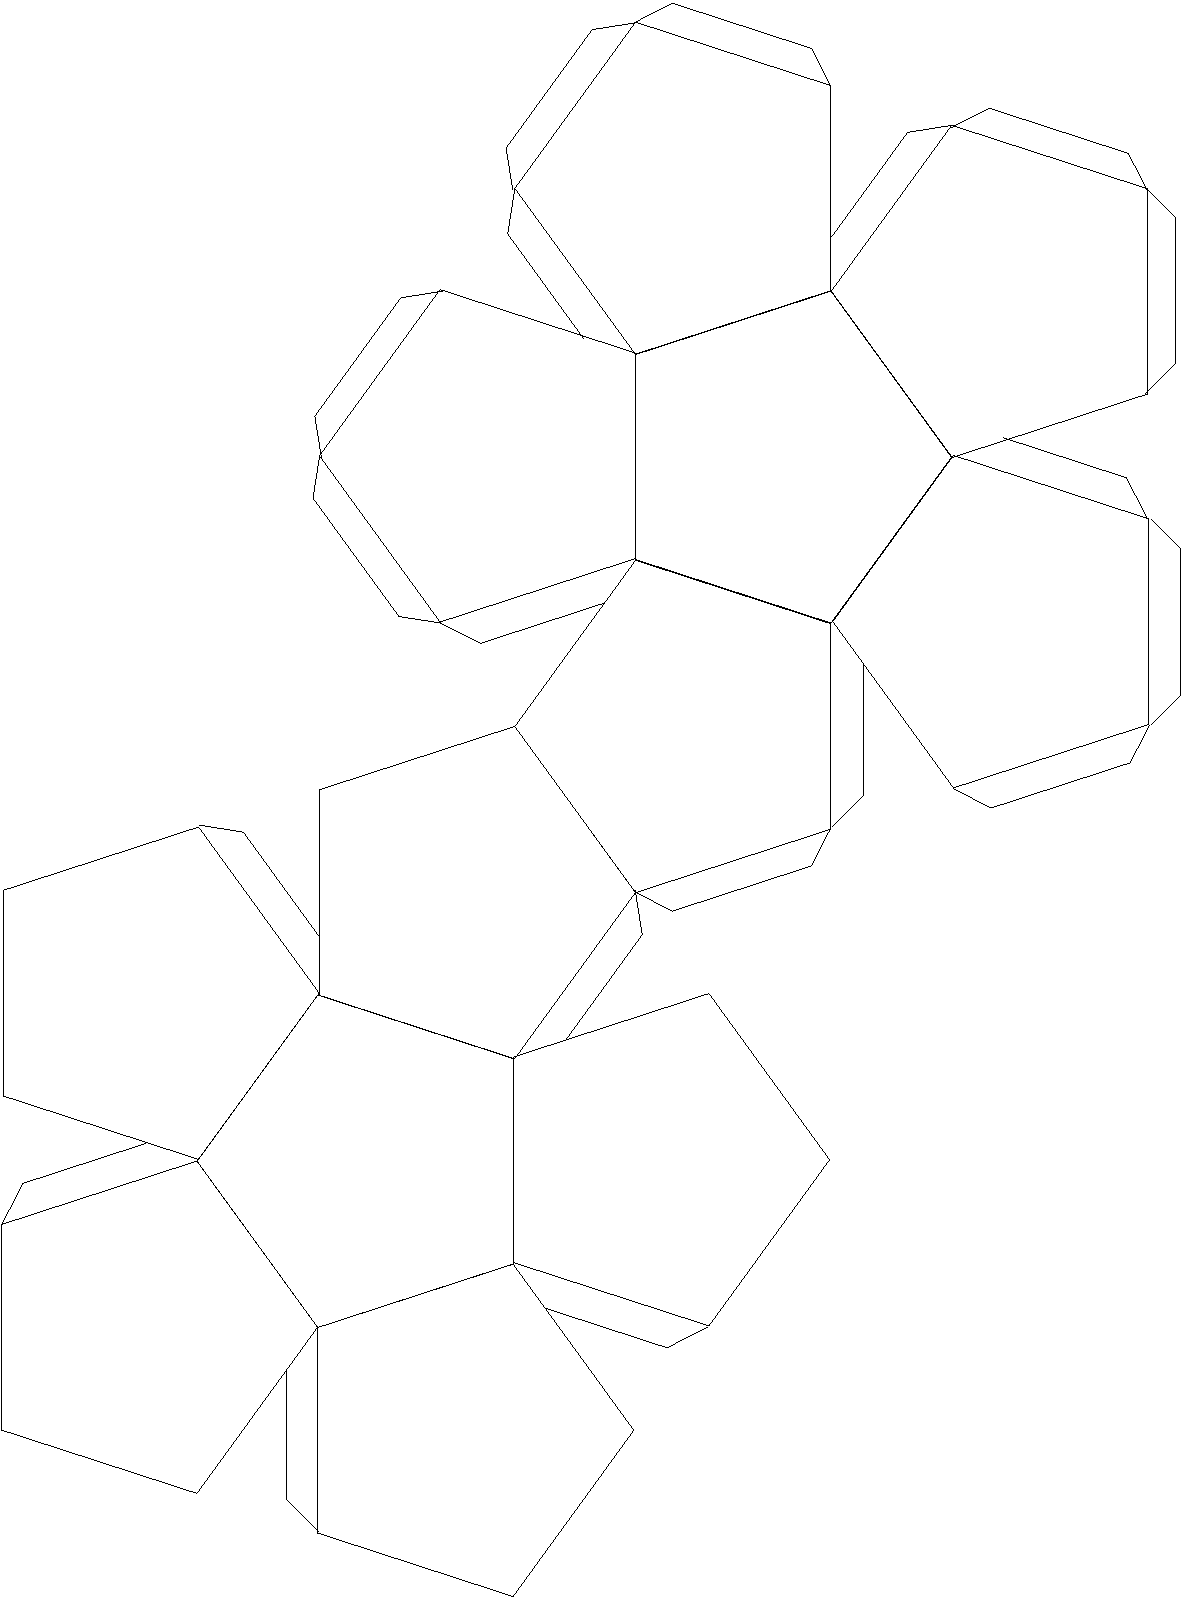
\includegraphics[scale=.5]{images/dodecahedron_template.pdf}}
\bigskip

\newpage

This is a net for the icosahedron:
\bigskip

\centerline{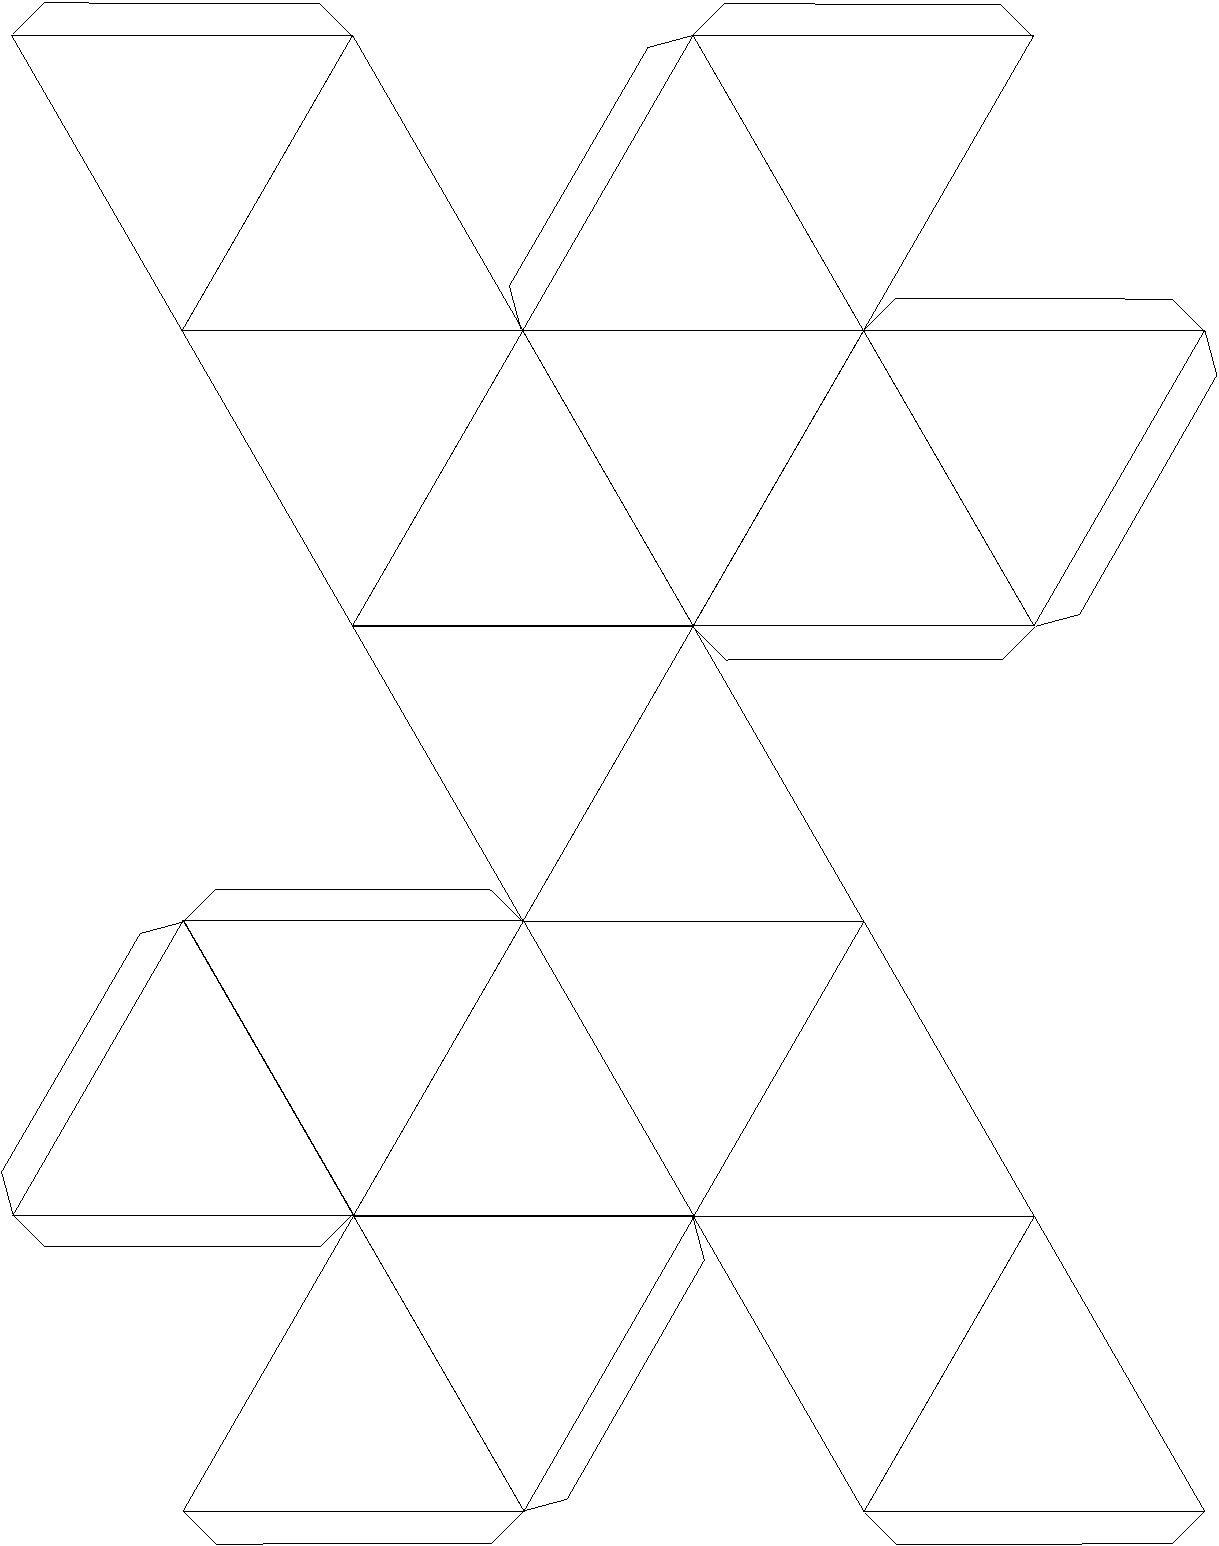
\includegraphics[scale=.5]{images/icosahedron_template.pdf}}
\bigskip

\newpage

You guessed it! It's time to completely finish the table!
\bigskip


\setlength{\tabcolsep}{18pt}
\begin{tabular}{r|c|c|c|c|c} 
\bigstrut name        & $F$ & $C$ & $F/C$ & $C/F$ & $E$ \\ \hline
\bigstrut tetrahedron & 4   & 4   & 3     & 3     & 6  \\ \hline
\bigstrut cube        & 6   & 8   & 3     & 4     & 12 \\ \hline
\bigstrut octahedron  & 8   & 6   & 4     & 3     & 12 \\ \hline
\bigstrut dodecahedron&     &     &       &       &    \\ \hline
\bigstrut icosahedron &     &     &       &       &    \\ \hline
\end{tabular}
\bigskip

Look carefully at your completed table.  Search for patterns.  Remember that weird switching around of 3's and 5's?  Mathematicians say that ``the tetrahedron is self-dual and the other platonic solids can be divided into pairs that are dual to one another.''  Any idea what they're talking about?

\newpage

\subsection{Exit Slip}

\begin{enumerate}
    \item What would you guess the Greek prefix {\em icosa} means?
    
    \wbvfill
    
    \item The word ``dozen'' literally means $2+10$.  How is this silly fact relevant to the naming of Platonic solids?
 
     \wbvfill
       
    \item Let's try some multi-counting.  Every one of the pentagons on a dodecahedron has 5 corners, and since there are 12 pentagonal faces that makes for $12 \cdot 5 \; = \; 60$ corners.  By what factor did we over-count the corners? \underline{\hstrut}
    
    How many corners are actually on a dodecahedron? \underline{\hstrut}

    \wbvfill
        
    \item Every face of a cube has 4 corners .  Since there are 6 faces on a cube, we get 
    $6 \cdot 4 = 24$ corners.  By what factor did we over-count the corners? \underline{\hstrut}
    
    How many corners are actually on a cube? \underline{\hstrut}
    
    \wbvfill
    
\end{enumerate}

\newpage

\subsection{Duals}

Look at the final table in the previous activity, and notice that there are some weird coincidences in the numbers.  For example, the dodecahedron and the icosahedron have the number of faces and the number of corners interchanged.  These coincidences lead to the idea of {\em duality}.

Which pairs of Platonic solids are dual to one another?

\wbvfill

Why is the tetrahedron called self-dual?

\wbvfill

You can make drawings of the platonic solids that lie flat in the plane, using some ideas from the mathematical area known as Topology.
(Topology means the study of shape.  Topologists study the things that remain the same even when an object is deformed somewhat.)

Imagine making a Platonic solid out of spaghetti noodles (maybe with meatballs holding the corners together).  Then (very carefully) cook your solid until the noodles get noodly. You should now be able to lay your ``solid'' out flat in the plane in such a way that no noodles cross each other.

Here's a wet noodle diagram of a cube:

\centerline{
\includegraphics[scale=.5]{images/wet_noodle_cube.png}}

\wbnewpage

\begin{enumerate}
    \item Make wet noodle diagrams of all 5 platonic solids.
    
    \wbvfill
    
    \item The corners of your Platonic solid are the points (meatballs) in the wet noodle diagram.  The edges of the solid are the noodles.  The faces of the Platonic solid have become regions in the plane surrounded/bordered by noodles.  Count the regions in each of your 5 noodle diagrams.
    
    \vspace{1in}
    
    \wbnewpage
    
    \item What happened to the missing faces?
    
    \wbvfill
    
    \item There is a process known as {\em truncation} that essentially means ``cut off the corners.''  Draw a wet noodle diagram for a truncated cube:
    
    \centerline{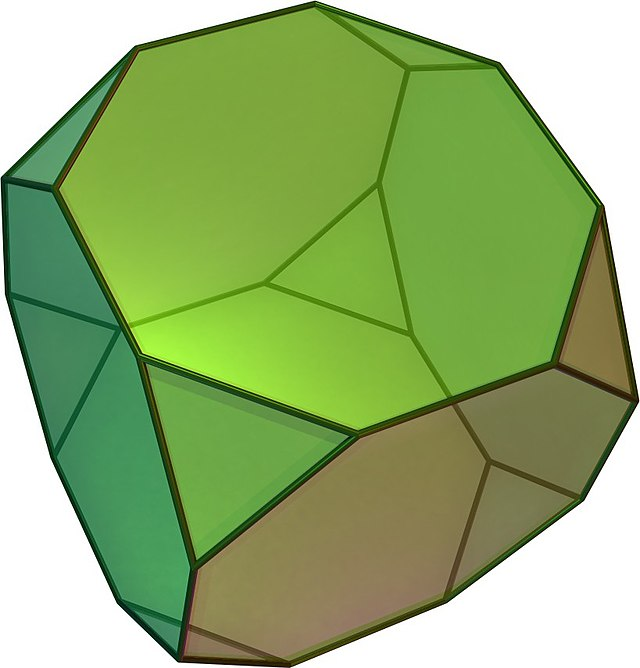
\includegraphics[scale=.25]{images/TruncatedCube.jpeg}}
    
    \wbvfill
    
    \item Now try making a wet noodle diagram for a truncated tetrahedron.
    
    \wbvfill
    
    \wbnewpage
    
    \item Try a wet noodle diagram of a 5-sided pyramid.
    
    \wbvfill
    
    \item Let's do some counting!  How many regions, edges and vertices (the fancy way to say `corners') are there in each of your diagrams?
    \bigskip
    
    Count the region outside your diagrams too when figuring out R.
    \bigskip
    
    \begin{tabular}{|r|c|c|c|}
    \strut name & R & E & V \\\hline
    \bigstrut tetrahedron & & & \\ \hline
    \bigstrut cube & & & \\ \hline
    \bigstrut octahedron & & & \\ \hline
    \bigstrut dodecahedron & & & \\ \hline
    \bigstrut icosahedron & & & \\ \hline
    \bigstrut truncated cube & & & \\ \hline
    \bigstrut truncated tetrahedron & & & \\ \hline
    \bigstrut pentagonal pyramid & & & \\ \hline
    \end{tabular}
\bigskip

    \item Make a fairly complicated, but random wet noodle diagram -- it doesn't need to actually come from something solid.  Find R, E, and V for your diagram.  What does $R-E+V$ equal?
    
    \wbvfill
    
   
   \wbnewpage
   
   \item For each of your Platonic solid noodle diagrams, draw a point somewhere in each region (don't forget to put a point on the outside!)  Connect points with a noodle if the corresponding regions are separated by a noodle.  It would be a good idea to make the original and the new diagram you're making be in different colors.  (BTW, this process is called {\em dualizing}).
   
   \wbvfill
   
\end{enumerate}

\wbnewpage

\subsection{Exit Slip}

\begin{enumerate}

\item Draw the WND and the dualized WND for a four-sided pyramid.

\wbvfill

    
    \item Fill in the blanks:
    
The dualized wet noodle diagram for the tetrahedron is a wet noodle diagram for a \underline{\rule{2in}{0pt}}

The dualized wet noodle diagram
for the cube is a wet noodle diagram for a(n) \underline{\rule{2in}{0pt}}.
    
 The dualized wet noodle diagram for the dodecahedron is a wet noodle diagram for a(n) \underline{\rule{2in}{0pt}}
    
    \item Verify the identity $R-E+V = 2$ for a soccer ball.
    
    \wbvfill
    
    
\end{enumerate}

\wbnewpage

%\subsection{Activity: into the 4th dimension}

\subsection{Project Choices}

\begin{enumerate}
    \item Make all five Platonic solids.
    
    You can make these models in many different ways:  3-d printing, plaited models (like the D4 we started this section with), paper nets can be assembled with glue and tabs, wire and wire nuts, pipecleaners, clay (or Play Doh), straws and paper clips, wood, solid gold or platinum, etc.
    
    \item Make 5 models that show the stages of a cube being transformed into an octahedron (or vice versa) via truncation.
    
    \item Make a calendar - a plaited model of a rhombic dodecahedron marked with a calendar for 2023 is available.
       
    \item The ``wet noodle diagrams'' we talked about are actually known as Planar Graphs.  Do some research and give a presentation on the K\"{o}nigsberg Bridge Problem and how this strange recreational problem lead to the area now known as Graph Theory.
        
    \item A flat plane and a sphere are hard to tell apart (ask any member of the Flat Earth Society).  The number we calculated R-E+V (which is usually rendered as V-E+F) is always 2 when your drawing is done on a plane or a sphere.  This is known as the Euler characteristic.  Demonstrate to your classmates that V-E+F need not be 2 if you make a drawing on the surface of a doughnut!
    
\end{enumerate}